\documentclass[12pt,twoside,openright]{book}
\usepackage[a4paper,top=22mm,bottom=22mm,left=25mm,right=25mm]{geometry}
\usepackage[T1]{fontenc}
\usepackage{lmodern}
\usepackage{amsmath,amssymb,amsfonts}
\usepackage{graphicx}
\usepackage{xcolor}
\usepackage{tikz}
\usepackage{pgfplots}
\pgfplotsset{compat=1.18}
\usetikzlibrary{
  shapes.geometric, shapes.misc, arrows.meta, positioning, calc,
  decorations.pathreplacing, decorations.markings, fit, backgrounds,
  matrix, shadows, patterns, chains, quotes, automata
}
\usepackage{listings}
\usepackage{booktabs}
\usepackage{array}
\usepackage{multirow}
\usepackage{longtable}
\usepackage{fancyhdr}
\usepackage{hyperref}
\usepackage{cleveref}
\usepackage{caption}
\usepackage{subcaption}
\usepackage{float}
\usepackage{enumitem}
\usepackage{tcolorbox}
\tcbuselibrary{listingsutf8,skins,breakable,fitting}
\usepackage{microtype}
\usepackage{setspace}
\usepackage{titlesec}
\usepackage{mdframed}
\usepackage{tabularx}
\usepackage{colortbl}
\usepackage{makecell}
\usepackage{makeidx}
\makeindex

\setlength{\headheight}{25pt}
\addtolength{\topmargin}{-8pt}

\definecolor{smartblue}{RGB}{0,82,155}
\definecolor{smartgreen}{RGB}{0,128,64}
\definecolor{smartorange}{RGB}{220,90,0}
\definecolor{smartred}{RGB}{180,30,30}
\definecolor{smartgray}{RGB}{80,80,80}
\definecolor{lightblue}{RGB}{220,235,250}
\definecolor{lightgreen}{RGB}{220,245,220}
\definecolor{lightorange}{RGB}{255,240,210}
\definecolor{lightred}{RGB}{255,220,220}
\definecolor{lightgray}{RGB}{245,245,245}
\definecolor{urllccolor}{RGB}{180,0,0}
\definecolor{embbcolor}{RGB}{0,100,180}
\definecolor{iotcolor}{RGB}{0,140,60}
\definecolor{codebg}{RGB}{248,248,248}
\definecolor{codeframe}{RGB}{180,180,200}

\lstdefinelanguage{Verilog}{
  morekeywords={module,endmodule,input,output,inout,wire,reg,always,assign,
    begin,end,if,else,case,casez,casex,endcase,for,generate,genvar,
    endgenerate,parameter,localparam,integer,posedge,negedge,initial,
    include,define,ifndef,endif,ifdef,function,endfunction,task,endtask},
  sensitive=true, morecomment=[l]{//}, morecomment=[s]{/*}{*/}, morestring=[b]"
}
\lstset{
  language=Verilog, basicstyle=\ttfamily\footnotesize,
  keywordstyle=\color{smartblue}\bfseries, commentstyle=\color{smartgreen}\itshape,
  stringstyle=\color{smartorange}, numberstyle=\tiny\color{smartgray},
  backgroundcolor=\color{codebg}, frame=single, framesep=3pt,
  rulecolor=\color{codeframe}, numbers=left, numbersep=8pt, stepnumber=1,
  breaklines=true, breakatwhitespace=true, tabsize=4, showstringspaces=false,
  xleftmargin=1.5em, xrightmargin=0.5em, captionpos=b, aboveskip=8pt, belowskip=8pt
}

\pagestyle{fancy}\fancyhf{}
\fancyhead[LE]{\small\leftmark}\fancyhead[RO]{\small\rightmark}
\fancyfoot[LE,RO]{\small\thepage}
\fancyfoot[CO,CE]{\small\textit{HA-TFF --- A Thesis on Line-Rate Hardware Firewalling}}
\renewcommand{\headrulewidth}{0.4pt}

\tcbset{
  defbox/.style={colback=lightblue,colframe=smartblue,fonttitle=\bfseries,title={Definition},arc=2pt,boxrule=0.6pt},
  warnbox/.style={colback=lightred,colframe=smartred,fonttitle=\bfseries,title={Design Note},arc=2pt,boxrule=0.6pt},
  notebox/.style={colback=lightgreen,colframe=smartgreen,fonttitle=\bfseries,arc=2pt,boxrule=0.6pt},
  keybox/.style={colback=lightorange,colframe=smartorange,fonttitle=\bfseries,title={Key Concept},arc=2pt,boxrule=0.6pt}
}

\hypersetup{colorlinks=true,linkcolor=smartblue,citecolor=smartgreen,urlcolor=smartorange,
  pdftitle={HA-TFF: A Hardware-Accelerated Telemetry Firewall for Line-Rate Packet Classification}}

\tikzset{every node/.append style={align=center}}
\tikzset{
  mod/.style={rectangle, draw=smartblue, fill=lightblue, thick, rounded corners=2pt,
    minimum width=30mm, minimum height=12mm, text centered, font=\tiny\bfseries,
    text width=30mm, align=center},
  io/.style={rectangle, draw=smartgray, fill=lightgray, thick, rounded corners=2pt,
    minimum width=22mm, minimum height=11mm, text centered, font=\tiny,
    text width=22mm, align=center},
  blk/.style={rectangle, draw=smartblue, fill=lightblue, thick,
    minimum width=20mm, minimum height=10mm, text centered, font=\tiny\bfseries,
    text width=20mm, align=center, rounded corners=2pt},
  reg/.style={rectangle, draw=smartred, fill=lightred, thick,
    minimum width=9mm, minimum height=10mm, font=\tiny, text centered,
    text width=9mm, align=center},
  st/.style={circle, draw=smartblue, fill=lightblue, thick,
    minimum size=15mm, font=\tiny\bfseries, text centered, text width=15mm, align=center},
  op/.style={circle, draw=smartorange, fill=lightorange, thick,
    minimum size=9mm, font=\tiny\bfseries, text centered, text width=9mm, align=center},
  seg/.style={rectangle, draw=smartblue, fill=lightblue, thick,
    minimum width=11mm, minimum height=8mm, font=\tiny, text centered, text width=11mm, align=center},
  bank/.style={rectangle, draw=smartblue, fill=lightblue, thick,
    minimum width=20mm, minimum height=42mm, text centered, font=\tiny\bfseries, text width=20mm, align=center},
  key/.style={rectangle, draw=smartred, fill=lightred, thick,
    minimum width=14mm, minimum height=8mm, font=\tiny, text centered, text width=14mm, align=center},
  p/.style={rounded rectangle, draw, thick, minimum width=55mm, minimum height=12mm,
    font=\tiny\bfseries, text centered, text width=55mm, align=center},
  box/.style={rectangle, draw=smartblue, fill=lightblue, thick,
    minimum width=8mm, minimum height=8mm, font=\tiny, text centered, text width=8mm, align=center},
  arrow/.style={->, >=Stealth, thick, smartblue},
  ctrl/.style={->, >=Stealth, thick, smartorange, dashed},
  lbl/.style={font=\tiny, text=smartgray, align=center, text width=44mm},
  albl/.style={font=\tiny, text=smartgray, align=center, text width=20mm},
  ev/.style={font=\tiny, text=smartgray, align=center, text width=50mm}
}

\begin{document}

% ═══════════════════════════════════════════════════════════════════════════
% FRONT MATTER
% ═══════════════════════════════════════════════════════════════════════════
\frontmatter

\begin{titlepage}
\begin{tikzpicture}[remember picture,overlay]
  \fill[smartblue] (current page.north west) rectangle ([yshift=-60mm]current page.north east);
  \fill[smartorange!80!black] ([yshift=20mm]current page.south west) rectangle ([yshift=25mm]current page.south east);
  \foreach \x in {0,15,...,210} {
    \draw[white!20!smartblue,very thin] ([xshift=\x mm]current page.north west) -- ([xshift=\x mm, yshift=-60mm]current page.north west);
  }
\end{tikzpicture}

\vspace*{15mm}
\begin{center}
{\color{white}\fontsize{24}{30}\selectfont\bfseries HA-TFF}\\[4mm]
{\color{white!80!smartblue}\fontsize{13}{17}\selectfont A Hardware-Accelerated Telemetry Firewall:\\
A High-Performance Packet Classification and\\Monitoring Engine for FPGA}\\[16mm]

\begin{tcolorbox}[colback=white,colframe=smartblue,arc=4pt,width=0.92\textwidth,boxrule=1pt]
{\large\color{smartgray} Pure-RTL 10\,GbE Exact-Match Classification with Keyed Anti-DoS Hashing,\\
Cuckoo Rule Tables, Integrated Telemetry, and Performance Monitoring}
\end{tcolorbox}

\vspace{16mm}
{\small\color{smartgray}
A thesis submitted in partial fulfilment of the requirements\\
for the degree of \textit{Master of Science in Computer Engineering}\\[4mm]
School of Electrical and Computer Engineering\\[4mm]
Based on the open-source repository: \texttt{https://github.com/ha-tff/ha-tff-fpga}}
\end{center}
\end{titlepage}

\cleardoublepage
\thispagestyle{empty}
\vspace*{40mm}
\begin{center}
{\Large\bfseries Declaration}
\end{center}
\vspace{8mm}
\noindent I declare that this thesis, entitled \emph{``HA-TFF: A Hardware-Accelerated Telemetry
Firewall for Line-Rate Packet Classification,''} is my own original work except where explicitly
cited. The design, implementation, verification, and analysis described herein were carried out by
the author. This work has not been submitted previously for any degree or professional qualification.

\vspace{10mm}
\begin{flushright}
\rule{60mm}{0.4pt}\\
\textit{The HA-TFF Engineering Team}\\
\today
\end{flushright}

\cleardoublepage
\thispagestyle{empty}
\vspace*{45mm}
\begin{center}
{\Large\bfseries Abstract}
\end{center}
\vspace{6mm}

\noindent This thesis presents the design, implementation, and evaluation of \textbf{HA-TFF}, a
pure-RTL hardware-accelerated telemetry firewall for FPGA. HA-TFF performs line-rate packet
classification and filtering for 10\,GbE networks while simultaneously providing comprehensive
hardware telemetry to a host CPU. The architecture integrates a keyed, hash-based exact-match
lookup engine using parallel Block-RAM (BRAM) banks, a four-way Cuckoo-hash rule table, and a
statistical telemetry engine. The system operates at 156.25\,MHz on an Artix-7 FPGA with a pipeline
latency of 16 clock cycles ($\approx 102.4$\,ns) and consumes minimal logic resources (811 LUTs,
1{,}608 registers). The design demonstrates the viability of FPGA-accelerated packet processing
with integrated monitoring for software-defined networking applications.

\vspace{4mm}
\noindent\textbf{Keywords:} FPGA, packet classification, firewall, telemetry, high-performance
networking, hardware acceleration, AXI4-Stream, Cuckoo hashing, network security.

\cleardoublepage
\thispagestyle{empty}
\vspace*{45mm}
\begin{center}
{\Large\bfseries Acknowledgements}
\end{center}
\vspace{6mm}
\noindent The author thanks the open-source hardware community whose prior work on AXI4 pipelining,
Cuckoo hashing, and FPGA telemetry established the foundations drawn upon here, and the maintainers
of the AMD/Xilinx Vivado toolchain whose synthesis and implementation reports made the timing and
resource analysis in this thesis possible.

\cleardoublepage
\thispagestyle{empty}
\tableofcontents
\cleardoublepage
\thispagestyle{empty}
\listoffigures
\cleardoublepage
\thispagestyle{empty}
\listoftables
\cleardoublepage
\thispagestyle{empty}
\section*{List of Acronyms}
\begin{tabular}{ll}
5-tuple & Source/dest IP, source/dest port, protocol \\
ADR & Architecture Decision Record \\
AXI & Advanced eXtensible Interface (AMBA) \\
BRAM & Block Random-Access Memory \\
COTS & Commercial Off-The-Shelf \\
DPU & Data Processing Unit \\
DV & Design Verification \\
FGG484 & Artix-7 484-ball package \\
FPGA & Field-Programmable Gate Array \\
FSM & Finite-State Machine \\
HA-TFF & Hardware-Accelerated Telemetry Firewall \\
INT & In-Band Network Telemetry \\
IOB & I/O Bond (bonded input/output) \\
LUT & Look-Up Table (FPGA logic) \\
Mpps & Million packets per second \\
SDN & Software-Defined Networking \\
SVA & SystemVerilog Assertions \\
TCAM & Ternary Content-Addressable Memory \\
WNS & Worst Negative Slack (timing) \\
\end{tabular}
\cleardoublepage

% ═══════════════════════════════════════════════════════════════════════════
% MAIN MATTER
% ═══════════════════════════════════════════════════════════════════════════
\mainmatter

% ======================================================================
% CHAPTER 1: INTRODUCTION
% ======================================================================
\chapter{Introduction}
\label{chap:intro}

\section{Motivation and Problem Statement}
\label{sec:motivation}

Modern networks operate at 10\,Gigabit Ethernet (10GbE) and beyond. A 10GbE link delivers
$10\times10^9$ bits per second; the smallest legal Ethernet frame consumes 672 bits on the wire
(64-byte frame + 8-byte preamble/SFD + 12-byte inter-packet gap). The worst-case arrival rate is

\begin{equation}
R_{\text{line}} = \frac{10\times10^9}{(64+8+12)\times 8}
                 = \frac{10^{10}}{672}
                 \approx 14.88\times 10^6\ \text{frames/s}.
\label{eq:lineratesec}
\end{equation}

\noindent Equivalently, a new frame arrives every

\begin{equation}
T_{\text{arr}} = \frac{1}{R_{\text{line}}} \approx 67.2\ \text{ns}.
\label{eq:arrival}
\end{equation}

This inter-arrival time is the fundamental budgeting constraint for any 10GbE classifier. It is
illustrated conceptually in Figure~\ref{fig:motivation}, which places HA-TFF on the data path
between the line interface and the host CPU.

\begin{figure}[H]
\centering
\footnotesize
\begin{tikzpicture}[node distance=14mm and 12mm]
  \node[blk] (nic) at (0,0) {10GbE NIC / MAC\\(line rate)};
  \node[blk, fill=lightorange!40, draw=smartorange] (hw) at (55mm,0) {HA-TFF\\(FPGA datapath)};
  \node[blk] (cpu) at (110mm,0) {Host CPU\\(telemetry consumer)};
  \node[blk, fill=lightgreen!40, draw=smartgreen] (tel) at (55mm,-18mm) {Telemetry\\(stats + perfmon)};
  \draw[arrow] (nic) -- (hw) node[midway, above, font=\tiny, text=smartgray] {AXI4-Stream in};
  \draw[arrow] (hw) -- (cpu) node[midway, above, font=\tiny, text=smartgray] {AXI4-Stream out};
  \draw[arrow, dashed, smartgreen] (hw) -- (tel);
  \draw[arrow, dashed, smartgreen] (tel) -| (cpu) node[midway, below, font=\tiny, text=smartgray] {AXI4-Lite};
  \node[ev] at (55mm,-32mm) {Line-rate classification \emph{and} observability in one pipeline.};
\end{tikzpicture}
\caption{Motivation: HA-TFF sits on the 10GbE path and exports telemetry to the host CPU without
breaking line rate.}
\label{fig:motivation}
\end{figure}

Software-based packet processing cannot meet this budget deterministically. A CPU core at 4\,GHz
executes only $\approx 270$ instructions in 67.2\,ns, far fewer than a robust classify-and-count
path requires once cache misses (50--75\,ns each) and OS scheduling jitter are accounted for: a
single last-level cache miss alone admits 7--11 new minimum-size frames. The challenge we address is
therefore twofold. First, the classification \emph{decision} must be rendered in hardware, with
fixed, bounded latency. Second, the \emph{observability} that a software firewall enjoys --- per
protocol counts, drop reasons, occupancy, and latency --- must be preserved, because a firewall
the operators cannot see is a firewall they cannot trust. HA-TFF answers both: a pure-RTL datapath
for the decision, and hardware telemetry engines for the visibility, integrated so that neither
compromises the other.

\section{Research Questions}

This thesis addresses four research questions, each revisited with evidence in
Chapter~\ref{chap:discussion}.

\begin{enumerate}[itemsep=4pt]
  \item[\textbf{RQ1}] Can an FPGA-based packet classification engine achieve line-rate processing
        for 10GbE traffic while maintaining deterministic latency? We hypothesise that a deeply
        pipelined, BRAM-backed exact-match engine can sustain 14.88\,Mpps with a fixed 16-cycle
        latency.
  \item[\textbf{RQ2}] How can hardware telemetry be integrated into a packet-processing pipeline
        without degrading performance? We hypothesise that observing existing AXI-Stream and
        datapath signals in parallel adds no critical-path logic.
  \item[\textbf{RQ3}] What are the resource, power, and performance trade-offs in implementing a
        keyed hash-based exact-match classification on FPGA? We quantify LUT/register/BRAM/DSP/IOB
        and power on an Artix-7.
  \item[\textbf{RQ4}] How does the system compare to alternative approaches (software firewalls,
        commercial FPGA SmartNICs, academic platforms) in throughput, latency, and resource
        utilisation? We compare against literature and known platforms.
\end{enumerate}

\section{Contributions}

This thesis makes the following contributions:

\begin{enumerate}[itemsep=3pt]
  \item \textbf{Complete RTL firewall with integrated telemetry.} A synthesizable, pure-RTL design
        spanning parser, keyed hash, Cuckoo BRAM table, matcher, delay-line synchronisation,
        statistics engine, and performance monitor.
  \item \textbf{Line-rate demonstration on entry-level FPGA.} Timing closure at 156.25\,MHz on an
        Artix-7 with $<2$\% logic and zero DSP usage.
  \item \textbf{Non-intrusive telemetry integration.} A methodology for stalls, occupancy, and
        latency histograms that leaves the critical datapath untouched.
  \item \textbf{Empirical evaluation.} Resource utilisation, timing closure, power, and functional
        correctness evidence.
  \item \textbf{Open-source release.} The full RTL is MIT-licensed and reproducible from the
        repository.
  \item \textbf{ADR-based documentation.} Engineering decisions captured as Architecture Decision
        Records for maintainability.
\end{enumerate}

\section{Thesis Organisation}

The remainder of this thesis is organised as follows. Chapter~\ref{chap:background} establishes the
foundations --- packet structure, AXI protocols, FPGA architecture, classification techniques, and
related work. Chapter~\ref{chap:architecture} presents the system architecture module by module,
with block diagrams, finite-state machines, and timing analyses.
Chapter~\ref{chap:implementation} covers module-level implementation and the ADR-driven design
rationale, including version history. Chapter~\ref{chap:verification} describes the dual
verification methodology. Chapter~\ref{chap:results} reports synthesis and performance evaluation,
with resource, timing, power, and comparison data. Chapter~\ref{chap:discussion} discusses the
results against the research questions and outlines future work.
Chapter~\ref{chap:conclusion} concludes. Appendices provide module documentation, the register map,
test vectors, synthesis reports, ADRs, bug reports, the golden model, and the RTL source.

% ======================================================================
% CHAPTER 2: BACKGROUND
% ======================================================================
\chapter{Background and Related Work}
\label{chap:background}

This chapter establishes the technical foundations upon which HA-TFF is built and positions the
design against prior art. We begin with the structure of the packets themselves, proceed through
the on-chip buses that carry them, survey the FPGA substrate, examine classification and hashing
techniques, and close with related work.

\section{Packet Processing Fundamentals}

\subsection{OSI Model and Network Packet Structure}

A classifier operates on the layered headers that precede a packet's payload. On a typical
Ethernet/IPv4/TCP (or UDP) flow the relevant fields are:

\begin{itemize}[itemsep=2pt]
  \item \textbf{Ethernet (14 bytes)}: destination MAC (6), source MAC (6), EtherType (2). An
        EtherType of \texttt{0x0800} denotes IPv4.
  \item \textbf{IPv4 (20 bytes, no options)}: version/IHL, differentiated services, total length,
        identification, flags/fragment offset, \emph{TTL}, \emph{protocol} (1 byte), header
        checksum, \emph{source address} (4 bytes), \emph{destination address} (4 bytes).
  \item \textbf{TCP/UDP (8 bytes for ports)}: \emph{source port} (2), \emph{destination port} (2),
        plus length/checksum or sequence/acknowledgement fields.
\end{itemize}

The \textbf{5-tuple} is the set (source IP, destination IP, source port, destination port,
protocol). It is the canonical identifier of a flow and the key HA-TFF hashes and matches. A crucial
geometric fact underpins the parser: the Ethernet + IPv4 + TCP/UDP header stack is 42 bytes, which
is smaller than the 64-byte AXI4-Stream beat. Consequently the \emph{entire} header stack is present
on the first beat, so the parser can extract the 5-tuple with purely combinatorial slicing and
requires no byte-by-byte state machine across beats. This is the single most important
simplification in the design and is why the parser is a small finite-state machine rather than a
general-purpose parser.

Parsing challenges in hardware include variable-length IPv4 options (IHL $>5$), VLAN tags
(\texttt{0x8100}), and tunneling. HA-TFF deliberately scopes itself to the common case
(EtherType \texttt{0x0800}, protocol TCP or UDP) and raises \texttt{parse\_error} on anything else,
which the firewall then drops --- a defensible default-deny posture.

\subsection{AXI4-Stream Protocol}
\label{sec:axi}

AXI4-Stream is a unidirectional, ready/valid handshaked bus defined by the AMBA specification
\cite{axi2017}. Its principal signals are \texttt{TDATA} (the payload word), \texttt{TKEEP} (a
per-byte valid mask), \texttt{TLAST} (end-of-frame), \texttt{TVALID} (producer ready), and
\texttt{TREADY} (consumer ready). A transfer of a beat occurs only when both \texttt{TVALID} and
\texttt{TREADY} are asserted on a rising clock edge; either side may deassert its signal to apply
backpressure or to idle the link.

\begin{figure}[H]
\centering
\footnotesize
\begin{tikzpicture}[>=Stealth, font=\tiny]
  \draw[->, thick] (0,0) -- (62mm,0) node[right, text=smartgray] {CLK};
  \foreach \x in {0,10,20,30,40,50} \draw[thick] (\x mm,2mm) -- (\x mm,-2mm);
  \foreach \x in {5,15,25,35,45} \draw[thick] (\x mm,0) -- (\x mm,2mm);
  \draw[smartblue, thick] (10mm,-9mm) -- (10mm,-15mm) -- (30mm,-15mm) -- (30mm,-9mm);
  \node[albl] at (20mm,-19mm) {TVALID};
  \draw[smartgreen, thick] (20mm,-25mm) -- (20mm,-31mm) -- (50mm,-31mm) -- (50mm,-25mm);
  \node[albl] at (35mm,-35mm) {TREADY};
  \fill[smartred!30] (20mm,-15mm) rectangle (30mm,-31mm);
  \draw[smartred, <->, thick] (20mm,-39mm) -- (30mm,-39mm) node[midway, below, font=\tiny, text=smartred] {transfer};
  \node[ev] at (40mm,-46mm) {A beat is legal only when TVALID and TREADY overlap on a clock edge.};
\end{tikzpicture}
\caption{AXI4-Stream ready/valid handshake. Backpressure arises when the receiver deasserts
\texttt{TREADY}.}
\label{fig:handshake}
\end{figure}

The handshake has direct consequences for a firewall. Because the decision is made several cycles
after the first beat, the firewall must either buffer the packet or hold \texttt{TREADY} low to
stall the producer while it computes. HA-TFF chooses the former (a 16-cycle delay line), keeping
\texttt{TREADY} asserted so it never backs pressure onto the MAC; this simplifies the timing
contract and keeps the ingress interface always accepting. The performance monitor, by counting
cycles where \texttt{TVALID} is high without \texttt{TREADY} (and the egress analogue), makes any
future backpressure visible.

\subsection{10GbE at 156.25\,MHz}

The 10GbE physical coding sublayer serialises 64-bit data words encoded with the 64b/66b line
code. Presented to the FPGA fabric as a 64-bit AXI4-Stream at 156.25\,MHz, the achieved rate is

\begin{equation}
156.25\ \text{MHz} \times 64\ \text{bits} = 10\,000\ \text{Mbps} = 10\ \text{Gbps}.
\label{eq:10g}
\end{equation}

\noindent The 6.4\,ns clock period is the budgeting quantum for every pipeline stage. Timing closure
at this frequency on an Artix-7 $-1$ speed grade is comfortable for the shallow combinational paths
HA-TFF uses, as Chapter~\ref{chap:results} confirms.

\section{FPGA Architecture Overview}

\subsection{FPGA Resources: LUTs, Registers, BRAM, DSPs}

An FPGA is a sea of configurable logic. \textbf{LUTs} (look-up tables, typically 6-input in
Artix-7) implement combinatorial logic and small distributed RAM/shift-registers. \textbf{Registers}
(flip-flops) hold sequential state and pipeline stages. \textbf{Block RAM} (BRAM) provides dense,
wide, dual-ported on-chip memory, ideal for rule tables. \textbf{DSP slices} accelerate
multiplication and MAC operations. HA-TFF uses LUTs, registers, and BRAM exclusively --- zero DSP
slices --- because its datapath is XOR/shift/compare logic, which is inherently DSP-free and thus
portable to the smallest devices.

\subsection{Artix-7 Series FPGA (\texttt{xc7a100tfgg484-1})}

The target device provides 63{,}400 LUTs, 126{,}800 registers, 135 Block-RAM tiles (36\,Kb each),
and 240 DSP slices, in the FGG484 package with 285 bonded I/Os. Artix-7 is AMD/Xilinx's
cost-optimised 28\,nm family; choosing an entry-level part deliberately demonstrates that line-rate
classification does not require a premium device. The $-1$ speed grade is the slowest, leaving the
most timing margin.

\subsection{AXI4-Lite Control Plane}

AXI4-Lite is the simplified, memory-mapped sibling of AXI4-Stream, with separate write
(\texttt{aw}/\texttt{w}/\texttt{b}) and read (\texttt{ar}/\texttt{r}) channels and no burst
support. HA-TFF exposes hash keys, enable bits, rule-programming registers, and all telemetry
counters through an AXI4-Lite slave. Because control transactions are rare relative to packet
arrival, the control plane places no timing burden on the data path.

\section{Packet Classification Techniques}

\subsection{Exact-Match vs. Range-Match Classification}

\textbf{Exact-match} tests equality of a field against a stored value; \textbf{range-match} tests
inclusion in an interval (e.g., ``destination port in $[1024,65535]$''). Exact-match is trivially
parallelisable in BRAM (one read, one comparison) but cannot express ranges; the software control
plane must therefore expand ranges into discrete rules. HA-TFF adopts exact-match (ADR-001) for
hardware simplicity and deterministic lookup.

\subsection{Hashing Approaches}

A hash maps a high-dimensional key (the 104-bit tuple) to a small index. Cryptographic hashes
(SHA-family) are secure but require many cycles and are unsuitable for line rate. Non-cryptographic
hashes (XOR-fold, CRC, Jenkins) are cheap. \textbf{Keyed hashing} mixes a secret so an adversary
cannot predict collisions --- essential against \emph{hash-flooding}, where an attacker forces many
keys into one bucket to degrade lookup to $O(n)$ \cite{crosby2003,ferguson2003}. HA-TFF's keyed
XOR-fold (ADR-003) is a deliberate middle ground: one-cycle latency, minimal logic, and sufficient
(though not cryptographic) resistance for anti-flooding.

\subsection{Cuckoo Hashing}
\label{sec:cuckoo}

Cuckoo hashing \cite{pagh2001} uses $k\ge 2$ independent hash functions. A key resides in
\emph{one} of its $k$ candidate buckets; lookup probes all $k$ buckets in parallel. Insertion may
evict and re-home existing keys (the ``cuckoo'' behaviour) until all keys settle, or declare
failure and rebuild. With $k$ banks of capacity $m$, insertion succeeds with high probability up to
a load factor that improves with $k$ \cite{fotakis2005}. HA-TFF uses $k=4$.

\begin{figure}[H]
\centering
\footnotesize
\begin{tikzpicture}[node distance=10mm and 14mm]
  \node[key] (k) {Key $K$};
  \node[bank, right=16mm of k] (b0) {Bank 0\\(seed $h_0$)};
  \node[bank, right=14mm of b0] (b1) {Bank 1\\(seed $h_1$)};
  \node[bank, right=14mm of b1] (b2) {Bank 2\\(seed $h_2$)};
  \node[bank, right=14mm of b2] (b3) {Bank 3\\(seed $h_3$)};
  \draw[arrow, smartorange] (k) -- (b0.west) node[midway, above, font=\tiny, text=smartorange] {$h_0(K)$};
  \draw[arrow, smartorange] (k) -- (b1.west) node[midway, above, font=\tiny, text=smartorange] {$h_1(K)$};
  \draw[arrow, smartorange] (k) -- (b2.west) node[midway, above, font=\tiny, text=smartorange] {$h_2(K)$};
  \draw[arrow, smartorange] (k) -- (b3.west) node[midway, above, font=\tiny, text=smartorange] {$h_3(K)$};
  \node[lbl] at (75mm,-30mm) {$K$ is stored in exactly ONE candidate bucket; the hardware reads all four banks in parallel and matches.};
\end{tikzpicture}
\caption{Cuckoo hashing with $k=4$ banks. The key occupies one of four candidate buckets; lookup is
a parallel four-way read.}
\label{fig:cuckoo}
\end{figure}

\subsection{Comparison of Approaches}

Table~\ref{tab:approaches} contrasts the principal classification structures. TCAM gives $O(1)$
ternary match but is power-hungry and scarce on FPGA; Bloom filters are compact but admit false
positives; decision trees scale logarithmically but are wide and slow. Cuckoo hashing delivers
$O(1)$ exact-match in commodity BRAM, at the cost of offline placement --- an acceptable trade for
HA-TFF.

\begin{table}[H]
\centering
\footnotesize
\begin{tabularx}{0.95\textwidth}{lXXX}
\toprule
\textbf{Approach} & \textbf{Lookup} & \textbf{Hardware cost} & \textbf{Drawback} \\
\midrule
TCAM & $O(1)$ ternary & very high power & scarce on FPGA \\
Bloom filter & $O(k)$ & low & false positives \\
Decision tree & $O(\log n)$ & medium & wide, slow \\
\textbf{Cuckoo (this work)} & \textbf{$O(1)$ parallel} & \textbf{BRAM only} & \textbf{offline placement} \\
\bottomrule
\end{tabularx}
\caption{Classification approach comparison. Cuckoo hashing gives $O(1)$ lookup in commodity BRAM.}
\label{tab:approaches}
\end{table}

\section{Network Telemetry}

Telemetry is the collection of operational measurements for visibility. In modern data centres and
SDN, standards such as In-Band Network Telemetry (INT) and languages such as P4 \cite{bosshart2014}
push measurement into the data plane. For a firewall, the key performance signals are:
\textbf{stalls} (valid without ready, revealing backpressure), \textbf{occupancy} (concurrent
in-flight packets, revealing congestion), and \textbf{latency} (cycles from ingress to egress
decision, revealing pipeline health). HA-TFF computes all three in hardware.

\section{Related Work}

Academic platforms such as NetFPGA \cite{lockwood2007} and P4-programmable switches
\cite{bosshart2014}, the OpenFlow paradigm \cite{mckeown2008}, and commercial DPUs/SmartNICs
\cite{smartnic2021} all demonstrate line-rate processing. However, few open-source 10GbE-grade
FPGA firewalls \emph{integrate} hardware telemetry as a first-class primitive. HA-TFF fills this
gap with a low-cost, MIT-licensed, fully synthesizable design, and documents its decisions through
ADRs so the result is reproducible and auditable.

% ======================================================================
% CHAPTER 3: ARCHITECTURE
% ======================================================================
\chapter{System Architecture}
\label{chap:architecture}

This chapter presents the HA-TFF architecture module by module. We begin with the overall
decomposition and design philosophy, then descend into each subsystem: parser, keyed hash, BRAM
Cuckoo table, matcher, pipeline synchronisation, statistics, performance monitor, and the AXI4-Lite
control plane.

\section{Overall System Design}

\subsection{High-Level Architecture Overview}

The top-level module \texttt{ha\_tff\_system\_top\_v005} integrates four subsystems: the datapath,
the AXI4-Lite control plane, the statistics engine, and the performance monitor. Figure~\ref{fig:top}
shows the decomposition and the data/control flow.

\begin{figure}[H]
\centering
\footnotesize
\begin{tikzpicture}[node distance=12mm and 13mm]
  \node[io] (rx) {AXI4-Stream In\\(10GbE MAC)};
  \node[mod, right=13mm of rx] (dp) {Datapath:\\Parser $\to$ Hash $\to$ BRAM $\to$ Matcher};
  \node[mod, fill=lightorange!40, draw=smartorange, right=13mm of dp] (dl) {Delay Line\\(16 cyc) +\\Decision FIFO};
  \node[io, right=13mm of dl] (tx) {AXI4-Stream Out\\(To Network)};
  \node[mod, below=16mm of dp] (cp) {AXI4-Lite\\Control Plane};
  \node[mod, fill=lightgreen!40, draw=smartgreen, left=16mm of cp] (st) {Statistics\\Engine};
  \node[mod, fill=lightgreen!40, draw=smartgreen, right=16mm of cp] (pm) {Performance\\Monitor};
  \draw[arrow] (rx) -- (dp);
  \draw[arrow] (dp) -- (dl);
  \draw[arrow] (dl) -- (tx);
  \draw[ctrl] (cp) -- (dp);
  \draw[ctrl] (dp) |- (st);
  \draw[ctrl] (rx) |- (pm);
  \draw[ctrl] (tx) |- (pm);
  \draw[ctrl] (st) -- (cp);
  \draw[ctrl] (pm) -- (cp);
\end{tikzpicture}
\caption{HA-TFF top-level architecture. The datapath makes the forward/drop decision; the delay line
re-aligns packet bytes to that decision; statistics and performance monitors observe both ingress
and egress and feed the AXI4-Lite control plane.}
\label{fig:top}
\end{figure}

\subsection{Dataflow and System Interfaces}

The data plane flows \texttt{s\_axis\_*} $\to$ parse/hash/bram/match $\to$ delay $\to$
\texttt{m\_axis\_*}. The parser's enable is gated by \texttt{control[1]}; when disabled, raw
packets stream straight through. The control plane (AXI4-Lite) loads the hash secret, enables
blocks, programs rules, resets statistics, and reads telemetry. These transactions may occur at any
time without stalling the streaming path, because the two planes share only quiescent control
signals.

\subsection{Design Philosophy and Trade-offs}

Three principles govern the design. (1) \emph{Default-deny}: a packet is forwarded only on an
explicit forward rule; otherwise it is dropped. (2) \emph{Hardware simplicity over flexibility}:
fixed 5-tuple exact-match, no wildcards. (3) \emph{Deterministic latency and strict plane
separation}: the data plane never waits on the control plane. These choices trade expressive power
for guaranteed line-rate behaviour and auditable correctness.

\section{Packet Parser (\texttt{ha\_tff\_parser\_v002})}

\subsection{Parser FSM Design}

The parser is a finite-state machine counting 64-bit words. Because the header stack fits one beat,
extraction completes in a few cycles. Figure~\ref{fig:parserfsm} shows the state graph. The FSM
begins in \texttt{IDLE}; on the first \texttt{tvalid} it moves through \texttt{WORD0}--\texttt{WORD3},
latching header fields at each step, and \texttt{WORD3} makes the valid/error decision from
EtherType and protocol. \texttt{tlast} returns to \texttt{IDLE}.

\begin{figure}[H]
\centering
\footnotesize
\begin{tikzpicture}[node distance=20mm and 16mm]
  \node[st] (idle) {IDLE};
  \node[st, right=of idle] (w0) {WORD0};
  \node[st, right=of w0] (w1) {WORD1};
  \node[st, right=of w1] (w2) {WORD2};
  \node[st, below=16mm of w2] (w3) {WORD3\\DECIDE};
  \node[st, fill=lightgreen!40, draw=smartgreen, right=of w3] (ok) {VALID};
  \node[st, fill=lightred!40, draw=smartred, left=of w3] (err) {ERROR};
  \draw[arrow] (idle) -- node[midway, above, font=\tiny, text=smartgray] {tvalid} (w0);
  \draw[arrow] (w0) -- (w1);
  \draw[arrow] (w1) -- (w2);
  \draw[arrow] (w2) -- (w3);
  \draw[arrow] (w3) -- node[midway, right, font=\tiny, text=smartgray, text width=18mm] {eth=IPv4 \& TCP/UDP} (ok);
  \draw[arrow] (w3) -- node[midway, left, font=\tiny, text=smartgray, text width=18mm] {otherwise} (err);
  \draw[arrow] (ok.south) .. controls (40mm,-42mm) and (-5mm,-42mm) .. node[midway, below, font=\tiny, text=smartgray] {tlast} (idle);
  \draw[arrow] (err.south) .. controls (-20mm,-42mm) and (-25mm,-10mm) .. (idle);
\end{tikzpicture}
\caption{Parser FSM. Five words are consumed; WORD3 makes the valid/error decision from EtherType and
protocol. \texttt{tlast} returns to IDLE. BUG-006 forced \texttt{parse\_error} to clear every
cycle and to flag short packets.}
\label{fig:parserfsm}
\end{figure}

\subsection{Header Extraction Logic}

Ethernet type detection (\texttt{0x0800} = IPv4) gates IPv4 header extraction; the protocol byte
selects TCP (\texttt{0x06}) or UDP (\texttt{0x11}); source/destination addresses and ports are
sliced from fixed word offsets to assemble the 104-bit tuple
$\{$\texttt{src\_ip, dst\_ip, src\_port, dst\_port, protocol}$\}$. The parser is therefore a set of
wire assignments gated by a word counter --- minimal logic, one registered stage.

\subsection{Error Handling}

Non-IPv4 packets, IPv4 options (IHL $>5$), short packets, and malformed headers raise
\texttt{parse\_error}. BUG-006 corrected a sticky-error bug: the original code failed to clear
\texttt{parse\_error} in the non-matching branch, so a single bad packet could poison all
subsequent traffic. The fix clears \texttt{parse\_error} every cycle and explicitly flags short
packets on \texttt{tlast}.

\section{Keyed Hash Engine (\texttt{ha\_tff\_hash\_v002})}

\subsection{Hash Function Design}

The 104-bit tuple is zero-padded to 128 bits, XORed with the 128-bit secret, and reduced by four
independent folds: a linear XOR-fold, a bit-reversed XOR-fold, and two shifted/mixed derivatives.
Each produces a 12-bit index. Figure~\ref{fig:hashblock} shows the data flow.

\begin{figure}[H]
\centering
\footnotesize
\begin{tikzpicture}[node distance=14mm and 12mm]
  \node[blk] (t) {104-bit\\tuple};
  \node[op, right=of t] (x) {$\oplus$};
  \node[blk, right=of x] (p) {secured\\payload $P$};
  \node[op, right=of p] (f0) {XOR-fold};
  \node[op, right=of f0] (f1) {bit-rev};
  \node[op, right=of f1] (f2) {shift};
  \node[op, right=of f2] (f3) {shift};
  \node[reg, right=of f0] (h0) {$h_0$};
  \node[reg, right=of f1] (h1) {$h_1$};
  \node[reg, right=of f2] (h2) {$h_2$};
  \node[reg, right=of f3] (h3) {$h_3$};
  \draw[arrow] (t) -- (x);
  \draw[arrow] (x) -- (p);
  \draw[arrow] (p) -- (f0);
  \draw[arrow] (p) -- (f1);
  \draw[arrow] (p) -- (f2);
  \draw[arrow] (p) -- (f3);
  \draw[arrow] (f0) -- (h0);
  \draw[arrow] (f1) -- (h1);
  \draw[arrow] (f2) -- (h2);
  \draw[arrow] (f3) -- (h3);
  \node[lbl] at (75mm,-26mm) {Four independent, secret-keyed folds $\to$ four Cuckoo bank indices.};
\end{tikzpicture}
\caption{Keyed hash engine. The secret-mixed tuple is folded four ways to address the four Cuckoo
banks. All four outputs are produced in a single registered stage.}
\label{fig:hashblock}
\end{figure}

\subsection{Security Considerations}

Keyed hashing with a 128-bit secret protects against hash-flooding: without the secret, an attacker
cannot steer bucket collisions (Section~\ref{sec:cuckoo}). The bit-reversed seed ensures independence
across the four views, so learning one fold's collisions reveals nothing about the others.

\subsection{Hardware Implementation}

The four folds are computed combinationally and registered in one cycle, adding negligible logic and
no DSP. The secret is loaded at runtime over AXI4-Lite, so the same bitstream can be re-keyed
without resynthesis.

\section{Rule Table and BRAM Banks (\texttt{ha\_tff\_bram\_bank})}

\subsection{Cuckoo Table Organisation}

Four parallel BRAM banks hold 4096 entries each (12-bit address) at 128-bit width. The entry format
is: \texttt{bit[127]} valid, \texttt{bit[126]} action, \texttt{bit[125:104]} protocol,
\texttt{bit[103:0]} the 104-bit tuple. With four banks, the table holds 16{,}384 candidate slots.

\subsection{BRAM Implementation}

Each bank instantiates a Xilinx Block RAM primitive (\texttt{RAMB36E1}), read-first, initialised
from a \texttt{.mem} file. The read address comes from one hash seed; writes are driven by the
AXI4-Lite rule-programming path, gated per-bank by \texttt{rule\_write\_bank}, so runtime rule
updates never touch the wrong bank.

\subsection{Table Management}

Cuckoo placement is computed offline in software; the hardware performs lookup only. Runtime
updates load entries via AXI4-Lite, enabling live rule refreshes without interrupting traffic.

\section{Exact-Match Matcher (\texttt{ha\_tff\_matcher\_v002})}

\subsection{Four-Way Parallel Comparison}

The matcher delays the tuple by three cycles to align with the BRAM read data, then performs four
parallel 104-bit equality comparisons qualified by each bank's valid bit. Figure~\ref{fig:matchpipe}
shows the pipeline.

\begin{figure}[H]
\centering
\footnotesize
\begin{tikzpicture}[node distance=22mm and 10mm]
  \node[blk] (d) {Tuple delay\\$\times$3};
  \node[blk, right=of d] (c) {Stage 1:\\4$\times$compare};
  \node[blk, fill=lightorange!40, draw=smartorange, right=of c] (r) {Stage 2:\\reduce +\\default-deny};
  \draw[arrow] (d) -- (c);
  \draw[arrow] (c) -- (r);
  \node[albl] at (45mm,-16mm) {3-cycle matcher latency, aligned to BRAM read.};
\end{tikzpicture}
\caption{Matcher pipeline. Tuple delay absorbs BRAM latency; stage~1 compares all four banks in
parallel; stage~2 reduces to a single verdict with default-deny.}
\label{fig:matchpipe}
\end{figure}

\subsection{Pipeline Stages and Decision Logic}

Stage~1 computes the comparisons; stage~2 reduces the four match/action signals to a single verdict,
defaulting to drop. The outputs are \texttt{match\_valid} and \texttt{action\_forward}; absent a
matching forward rule, the packet is dropped (default-deny). Because the comparison is qualified by
the per-bank valid bit, an empty or stale entry can never falsely match.

\section{Pipeline Synchronisation}

\subsection{Data Delay Line (\texttt{axi\_stream\_delay\_line})}

A parameterised 16-cycle shift register delays packet bytes so they emerge aligned with the
decision. It is purely structural and adds no control logic to the data path.

\subsection{Decision FIFO}

A 32-deep, one-bit-wide FIFO stores the per-packet verdict, decoupling verdict production (matcher)
from consumption (delay-line output) and preserving order under backpressure. Figure~\ref{fig:decfifo}
illustrates the operation.

\begin{figure}[H]
\centering
\footnotesize
\begin{tikzpicture}[node distance=12mm]
  \draw[thick] (0,-5mm) rectangle (50mm,5mm);
  \node[box] at (10mm,0) {1};
  \node[box] at (20mm,0) {0};
  \node[box] at (30mm,0) {1};
  \node[box] at (40mm,0) {1};
  \node[lbl] at (25mm,12mm) {Decision FIFO (32 deep, 1 bit)};
  \draw[arrow, smartred] (0,0) -- (-14mm,0) node[midway, above, font=\tiny, text=smartred] {push verdict};
  \draw[arrow, smartgreen] (50mm,0) -- (64mm,0) node[midway, above, font=\tiny, text=smartgreen] {pop on new pkt};
  \node[lbl] at (25mm,-14mm) {Order-preserving: packet $i$'s verdict dequeued exactly when delayed packet $i$ emerges.};
\end{tikzpicture}
\caption{Decision FIFO operation. Verdicts are enqueued in packet order and dequeued in lockstep
with the delayed data stream.}
\label{fig:decfifo}
\end{figure}

\subsection{Pipeline Latency Analysis}

The decision latency is the sum of stage latencies:

\begin{equation}
L_{\text{dec}} = L_{\text{hash}} + L_{\text{bram}} + L_{\text{match}} = 1 + 2 + 3 = 6\ \text{cycles}.
\label{eq:dec}
\end{equation}

\noindent The delay line provides $L_{\text{delay}} = 16$ cycles, comfortably exceeding
$L_{\text{dec}}$ (BUG-008 corrected an earlier 6-cycle line that was too short). End-to-end latency
is fixed at $16 \times 6.4\ \text{ns} = 102.4\ \text{ns}$. Figure~\ref{fig:latency} shows the budget.

\begin{figure}[H]
\centering
\footnotesize
\begin{tikzpicture}[node distance=20mm and 8mm]
  \node[blk] (p) {Parse\\1};
  \node[blk, right=of p] (h) {Hash\\1};
  \node[blk, right=of h] (b) {BRAM\\2};
  \node[blk, right=of b] (m) {Match\\3};
  \node[blk, fill=lightorange!40, draw=smartorange, right=of m] (d) {Delay\\16};
  \draw[arrow] (p) -- (h); \draw[arrow] (h) -- (b); \draw[arrow] (b) -- (m); \draw[arrow] (m) -- (d);
  \draw[decorate, decoration={brace, amplitude=4pt}, smartred, thick]
    ($(p.north west)+(0,3mm)$) -- ($(m.north east)+(0,3mm)$)
    node[midway, above, font=\tiny, text=smartred, text width=30mm] {Decision = 6 cycles};
  \draw[decorate, decoration={brace, amplitude=4pt}, smartgreen, thick]
    ($(d.north west)+(0,3mm)$) -- ($(d.north east)+(0,3mm)$)
    node[midway, above, font=\tiny, text=smartgreen, text width=20mm] {Delay = 16};
  \node[lbl] at (52mm,-18mm) {Total deterministic latency = 16 cycles = 102.4 ns (fixed, zero jitter).};
\end{tikzpicture}
\caption{Latency budget. The 6-cycle decision path is shorter than the 16-cycle delay line,
guaranteeing correct verdict-to-packet re-alignment.}
\label{fig:latency}
\end{figure}

\section{Statistics Engine (\texttt{ha\_tff\_statistics})}

\subsection{Counter Architecture and Accumulation Logic}

The engine maintains RX/TX packet counters (32-bit), RX/TX byte counters (64-bit, accumulated from
the \texttt{tkeep}-derived valid-byte count each cycle), per-protocol counts (TCP, UDP, ICMP),
parse-error count, and drop count. Packet counters increment on \texttt{tlast}; byte counters
accumulate every cycle that \texttt{tvalid \&\& tready}; the drop counter increments when
\texttt{match\_valid \&\& !action\_forward}. All are readable via AXI4-Lite.

\subsection{Reset and Clear Semantics}

A self-clearing \texttt{control[2]} bit resets all counters synchronously without affecting packet
flow, so software can sample deltas over a window.

\section{Performance Monitor (\texttt{ha\_tff\_performance\_monitor})}

\subsection{Stall Detection}

\texttt{rx\_stalls} counts cycles where \texttt{TVALID} is high without \texttt{TREADY};
\texttt{tx\_stalls} counts the egress analogue. These reveal backpressure from the upstream MAC or
downstream network.

\subsection{Occupancy Tracking}

\texttt{current\_occupancy} counts concurrent in-flight packets; \texttt{peak\_occupancy} latches
the running maximum. BUG-007 separated occupancy from latency measurement, which had previously
coupled unrelated logic and produced incorrect peaks.

\begin{figure}[H]
\centering
\footnotesize
\begin{tikzpicture}[>=Stealth, font=\tiny]
  \draw[->, thick] (0,0) -- (110mm,0) node[right, text=smartgray] {Time};
  \draw[->, thick, smartgreen] (0,-6mm) -- (110mm,-6mm) node[right, text=smartgray] {active\_packets};
  \draw[thick, smartblue] (10mm,-6mm) -- (10mm,-18mm) -- (25mm,-18mm) -- (25mm,-12mm)
    -- (45mm,-12mm) -- (45mm,-24mm) -- (70mm,-24mm) -- (70mm,-9mm) -- (90mm,-9mm) -- (90mm,-15mm)
    -- (100mm,-15mm) -- (100mm,-6mm);
  \draw[thick, smartred, dashed] (0,-32mm) -- (110mm,-32mm) node[right, text=smartgray] {peak (latched)};
  \draw[thick, smartred] (45mm,-32mm) -- (45mm,-24mm);
  \node[lbl] at (55mm,-40mm) {Occupancy steps up on RX start, down on TX end; peak latches the maximum.};
\end{tikzpicture}
\caption{Occupancy waveform. \texttt{active\_packets} tracks in-flight packets; \texttt{peak\_occupancy}
latches the running maximum until stats reset.}
\label{fig:occupancy}
\end{figure}

\subsection{Latency Histogram}

A three-bin histogram ($<10$, $10\text{--}20$, $>20$ cycles) records per-packet latency. The current
model uses a single in-flight timer (a known simplification; a timestamp FIFO is future work).

\section{Control Plane (\texttt{ha\_tff\_axi\_lite\_regs})}

\subsection{AXI4-Lite Implementation and Control Flow}

The slave handles read/write transactions by decoding \texttt{awaddr}/\texttt{araddr} on bits
\texttt{[7:2]}. Rule programming writes four words then pulses \texttt{rule\_ctrl}; the stats reset
is self-clearing; firewall enable/disable is immediate. The full register map is in
Appendix~\ref{app:regmap}.

% ======================================================================
% CHAPTER 4: IMPLEMENTATION & DESIGN DECISIONS
% ======================================================================
\chapter{Implementation and Design Decisions}
\label{chap:implementation}

This chapter descends from architecture to register-transfer detail. We first survey each module's
implementation, then record the Architecture Decision Records that justify the key choices, and
close with the version history that produced the current design.

\section{Module-Level Implementation Details}

\subsection{Parser Implementation}

The parser is a word-count-driven FSM with a small set of registered outputs. Header fields are
sliced from fixed word offsets; the BUG-006 clear-every-cycle discipline prevents sticky errors.
The parser asserts \texttt{tuple\_valid} combinatorially-gated and \texttt{parse\_error} otherwise,
both re-registered for timing.

\subsection{Hash Implementation}

The bit-reversal is a 128-bit \texttt{generate} loop; the XOR-reduction network folds the
secret-mixed payload; seeds 2 and 3 are derived by shift/mix so all four indices differ. All four
folds share the same secured payload, so the logic is a few levels of XOR/shift --- trivially fast.

\subsection{BRAM Instantiation}

Each bank is a parameterised \texttt{RAMB36E1} with \texttt{INIT\_FILE} pointing at
\texttt{sim/bank*.mem}. Read and write ports are used for lookup and AXI4-Lite programming;
per-bank write-enable gating ensures atomic, correctly-targeted updates.

\subsection{Delay Line and Decision FIFO Implementation}

The delay line is a parameterised shift register of depth \texttt{LATENCY}; the Decision FIFO uses
a 32-entry one-bit memory with separate write/read pointers and an empty flag, guaranteeing
order-preserving association even under bursty traffic (BUG-008).

\subsection{Statistics Implementation}

Packet counters use 32-bit width; byte counters use 64-bit width; all increments are pipelined and
gated by \texttt{stats\_reset}. Because the counters are in the same clock domain as the datapath,
no CDC logic is required.

\section{Architecture Decision Records (ADRs)}

\subsection{ADR-001: Exact-Match Over Range-Match}
\textbf{Problem:} need arbitrary packet filtering. \textbf{Decision:} exact-match on the 5-tuple.
\textbf{Rationale:} hardware simplicity, deterministic lookup. \textbf{Consequence:} ranges must be
expanded to discrete rules in software.

\subsection{ADR-002: Cuckoo Hashing Over TCAM}
\textbf{Problem:} need line-rate lookup. \textbf{Decision:} Cuckoo hashing with four parallel banks.
\textbf{Rationale:} zero DSP usage, low power, BRAM availability. \textbf{Consequence:} offline rule
placement required.

\subsection{ADR-003: Keyed XOR Hashing Over Cryptographic Hash}
\textbf{Problem:} need a 10GbE hash resistant to flooding. \textbf{Decision:} simple XOR-fold with
128-bit key. \textbf{Rationale:} one-cycle latency, minimal logic. \textbf{Consequence:} not
cryptographically secure, but sufficient for anti-flooding.

\subsection{ADR-004: Default-Deny Security Posture}
\textbf{Problem:} firewall default behaviour. \textbf{Decision:} drop all packets without an
explicit forward rule. \textbf{Rationale:} security best practice. \textbf{Consequence:} rules must
be loaded before traffic passes; override via enable bit.

\subsection{ADR-005: 16-Cycle Pipeline Latency}
\textbf{Problem:} need to align decision with data. \textbf{Decision:} fixed 16-cycle delay line.
\textbf{Rationale:} timing closure at 156.25\,MHz with margin. \textbf{Consequence:} fixed
processing latency, no variable-latency features.

\section{Version History and Design Evolution}

The design evolved across twelve iterations: \textbf{v001--v002} established parser and 5-tuple
extraction; \textbf{v003--v004} added the keyed hash and BRAM Cuckoo banks; \textbf{v004--v005}
integrated the matcher, delay line, and system top; \textbf{+telemetry} added the statistics engine
and AXI-Lite extension; \textbf{+perf\_mon} added the performance monitor and resolved the IOB
constraint by migrating the target package from CSG324 to FGG484. Each iteration is captured in the
repository history and informed the ADRs above.

% ======================================================================
% CHAPTER 5: VERIFICATION
% ======================================================================
\chapter{Verification Methodology}
\label{chap:verification}

A line-rate hardware classifier is only trustworthy if its correctness is demonstrated, not assumed.
This chapter describes a two-tier verification strategy: a lightweight legacy Verilog testbench and
a modern SystemVerilog constrained-random environment with assertions, coverage, and a golden
model.

\section{Simulation-Based Verification}

\subsection{Legacy Testbench (\texttt{tb\_ha\_tff\_system\_top.v})}

An Icarus-Verilog-compatible testbench clocks the design at 156.25\,MHz, programs the hash secret
and a forward rule over AXI4-Lite, injects a hand-crafted TCP packet, and reads back telemetry. It
is the lowest-friction smoke test and runs in any open-source simulator.

\subsection{SystemVerilog DV Environment}

The \texttt{dv/} suite provides a constrained-random environment with a packet generator, monitors,
a scoreboard, and functional coverage. Figure~\ref{fig:dv} shows the structure.

\begin{figure}[H]
\centering
\footnotesize
\begin{tikzpicture}[node distance=12mm and 14mm]
  \node[mod] (gen) {Packet Generator\\(random + errors)};
  \node[mod, right=24mm of gen] (uut) {DUT\\ha\_tff\_system\_top\_v005};
  \node[mod, fill=lightgreen!40, draw=smartgreen, below=14mm of gen] (cov) {Coverage\\Collector};
  \node[mod, fill=lightred!40, draw=smartred, below=14mm of uut] (sva) {SVA\\Binder};
  \node[mod, fill=lightorange!30, draw=smartorange, below=24mm of cov] (gold) {Golden Model\\(Python)};
  \draw[arrow] (gen) -- (uut);
  \draw[arrow] (uut) -- (cov);
  \draw[arrow] (uut) -- (sva);
  \draw[arrow, smartorange, dashed] (gold) -- (cov);
  \node[lbl] at (50mm,-40mm) {Random stimulus + SVA assertions bound into the DUT + coverage; golden model for offline checks.};
\end{tikzpicture}
\caption{SystemVerilog DV environment: random stimulus, SVA assertions bound into the DUT, a coverage
collector, and an offline golden model.}
\label{fig:dv}
\end{figure}

\subsection{Directed and Random Test Cases}

Directed tests exercise protocol and error variations; random tests stress backpressure, short
packets, back-to-back packets, and \texttt{tlast} alignment. Together they exercise the corner
cases where the synchronisation logic is most fragile.

\section{Formal Verification (SVA)}

\subsection{AXI4-Stream, Parser, and Decision Assertions}

Concurrent assertions check protocol compliance (handshake, \texttt{tlast} timing, \texttt{tkeep}
validity), parser tuple-extraction completeness, parse-error conditions, and the invariant that
every valid packet is forwarded or dropped with a consistent counter increment. These catch
protocol violations that directed tests might miss.

\section{Functional Coverage}

Covergroups capture protocol (TCP/UDP/ICMP/IPv4), error, decision, and pipeline-state coverage,
including cross-coverage of combinations, giving quantitative confidence that the stimulus space
was adequately explored.

\section{Golden Model Validation}

\texttt{dv/golden\_model.py} (scapy-based) parses $\to$ hashes $\to$ looks up $\to$ decides $\to$
counts, computing expected telemetry for comparison against the RTL. Automating this comparison is
future work (Chapter~\ref{chap:discussion}).

\section{Bug Reports and Fixes}

\begin{table}[H]
\centering
\footnotesize
\begin{tabular}{llp{58mm}}
\toprule
\textbf{ID} & \textbf{Title} & \textbf{Fix} \\
\midrule
BUG-001 & Tuple Valid Timeout & Added reset/timeout on \texttt{tlast} \\
BUG-006 & Sticky Parse Error & Clear \texttt{parse\_error} each cycle; short-packet handling \\
BUG-007 & Occupancy Tracker Flaw & Separated occupancy from latency measurement \\
BUG-008 & Pipeline Synchronisation & Increased delay to 16 cycles; added Decision FIFO \\
\bottomrule
\end{tabular}
\caption{Key bug fixes. Each corrected a correctness defect in the synchronisation or error path.}
\label{tab:bugs}
\end{table}

% ======================================================================
% CHAPTER 6: SYNTHESIS RESULTS
% ======================================================================
\chapter{Synthesis Results and Performance Evaluation}
\label{chap:results}

This chapter reports the empirical evaluation of HA-TFF: synthesis methodology, resource
utilisation, timing closure, power, performance metrics, and a comparison with alternative
approaches. All numbers are from Vivado 2026.1 on \texttt{xc7a100tfgg484-1}.

\section{Synthesis Methodology}

\subsection{Target Device and Toolchain}

Xilinx Vivado 2026.1 targets \texttt{xc7a100tfgg484-1} at 156.25\,MHz ($-1$ speed grade). The
\texttt{synth.tcl} batch script elaborates the RTL, synthesises \texttt{ha\_tff\_system\_top\_v005},
and emits utilisation, timing, and power reports plus a checkpoint.

\subsection{Reports Generated}

The committed artefacts are \texttt{utilization\_report.txt}, \texttt{timing\_summary.txt},
\texttt{power\_report.txt}, and \texttt{ha\_tff\_system\_top\_v005\_synth.dcp} under
\texttt{reports/} (Appendix~\ref{app:reports}).

\section{Resource Utilisation}

\subsection{Overall Resource Consumption}

Table~\ref{tab:util} summarises utilisation. Logic is negligible ($<2$\%); BRAM dominates because of
the four 4096$\times$128b banks; IOB reflects the wide AXI buses.

\begin{table}[H]
\centering
\footnotesize
\begin{tabular}{lrrr}
\toprule
\textbf{Resource} & \textbf{Used} & \textbf{Available} & \textbf{Util \%} \\
\midrule
Slice LUTs & 811 & 63{,}400 & 1.28 \\
Slice Registers & 1{,}608 & 126{,}800 & 1.27 \\
Block RAM (36Kb) & 48 & 135 & 35.56 \\
DSP Slices & 0 & 240 & 0.00 \\
Bonded IOB & 241 & 285 & 84.56 \\
\bottomrule
\end{tabular}
\caption{HA-TFF resource utilisation (Vivado 2026.1, Artix-7 xc7a100tfgg484-1, 156.25\,MHz).}
\label{tab:util}
\end{table}

\subsection{Analysis by Module and Scaling}

The BRAM banks account for all 48 tiles; the parser, hash, matcher, delay line, statistics, and
performance monitor together use the 811 LUTs and 1{,}608 registers. Table size scales linearly with
BRAM: four banks $\times$ 4096 entries = 16{,}384 slots. Larger tables are feasible on devices with
more BRAM at unchanged logic cost. Figure~\ref{fig:utilchart} visualises the breakdown.

\begin{figure}[H]
\centering
\footnotesize
\begin{tikzpicture}
\begin{axis}[
  ybar, ymin=0, ymax=40, width=105mm, height=55mm,
  symbolic x coords={LUTs, Regs, BRAM, DSP, IOB},
  xtick=data, ylabel={Utilisation (\%)}, bar width=13mm,
  nodes near coords, nodes near coords style={font=\tiny},
  title={Resource Utilisation by Type}, title style={font=\small\bfseries}
]
  \addplot[fill=smartgreen] coordinates {(LUTs,1.28)(Regs,1.27)(BRAM,35.56)(DSP,0)(IOB,84.56)};
\end{axis}
\end{tikzpicture}
\caption{Resource utilisation. BRAM and IOB dominate; logic and DSP are negligible --- the design is
memory- and pin-bound, not logic-bound.}
\label{fig:utilchart}
\end{figure}

\section{Timing Analysis}

\subsection{Timing Closure at 156.25\,MHz}

Worst negative slack (WNS) is $+0.339$\,ns with zero failing endpoints; hold slack $+0.070$\,ns;
pulse-width slack $+1.950$\,ns. All constraints are met.

\subsection{Critical Path Analysis}

The critical path runs from a BRAM output through a nine-level CARRY4 comparator chain to the
matcher register (5.7\,ns data delay within the 6.4\,ns budget). Figure~\ref{fig:critical} shows it.

\begin{figure}[H]
\centering
\footnotesize
\begin{tikzpicture}[node distance=24mm and 8mm]
  \node[blk] (bram) {BRAM out\\(DOBDO[4])};
  \node[blk, right=of bram] (carry) {CARRY4\\(9 levels)};
  \node[blk, fill=lightorange!40, draw=smartorange, right=of carry] (ff) {Matcher reg\\(s1\_b0\_match)};
  \draw[arrow, smartred] (bram) -- node[midway, above, font=\tiny, text=smartred] {2.45 ns} (carry);
  \draw[arrow, smartred] (carry) -- node[midway, above, font=\tiny, text=smartred] {3.25 ns} (ff);
  \node[lbl] at (52mm,-16mm) {Total data path = 5.7 ns; slack = 0.339 ns @ 6.4 ns period.};
\end{tikzpicture}
\caption{Critical timing path: BRAM output $\to$ nine-level CARRY4 comparator $\to$ matcher
register.}
\label{fig:critical}
\end{figure}

\subsection{Power Consumption}

Estimated on-chip power is 0.159\,W (0.066\,W dynamic, 0.093\,W static). The I/O bank is the
largest dynamic contributor (0.034\,W), reflecting the wide interfaces. Figure~\ref{fig:powerchart}
breaks it down.

\begin{figure}[H]
\centering
\footnotesize
\begin{tikzpicture}
\begin{axis}[
  ybar, ymin=0, width=105mm, height=52mm,
  symbolic x coords={Clocks, Slice, Signals, BRAM, I/O, Static},
  xtick=data, ylabel={Power (W)}, bar width=11mm,
  nodes near coords, nodes near coords style={font=\tiny},
  title={On-Chip Power Breakdown (0.159 W total)}, title style={font=\small\bfseries}
]
  \addplot[fill=smartorange] coordinates
    {(Clocks,0.023)(Slice,0.002)(Signals,0.003)(BRAM,0.001)(I/O,0.034)(Static,0.093)};
\end{axis}
\end{tikzpicture}
\caption{Power breakdown. Static dominates; among dynamic contributors, the I/O bank is largest.}
\label{fig:powerchart}
\end{figure}

\section{Performance Metrics}

\subsection{Throughput, Latency, and Scalability}

The pipeline accepts one packet per clock, yielding 156\,Mpps capacity versus the 14.88\,Mpps 10GbE
minimum-frame requirement --- over $10\times$ headroom. Latency is deterministic at 16 cycles
($102.4$\,ns). The rule table holds 16{,}384 entries and scales with BRAM.

\section{Comparison with Related Work}

Table~\ref{tab:compare} compares HA-TFF with software firewalls, commercial FPGA SmartNICs, and
academic platforms. HA-TFF matches line rate at a fraction of the power and cost while providing
first-class hardware telemetry.

\begin{table}[H]
\centering
\footnotesize
\begin{tabularx}{0.95\textwidth}{lXXX}
\toprule
\textbf{Dimension} & \textbf{Software firewall} & \textbf{Commercial FPGA} & \textbf{HA-TFF} \\
\midrule
Throughput & $<$1\,Gbps & 10\,Gbps+ & 10\,Gbps \\
Latency & $\mu$s & $\sim$100\,ns & 102.4\,ns \\
Flexibility & high & medium & low (fixed rules) \\
Telemetry & rich (slow) & vendor-specific & hardware, AXI4-Lite \\
Cost & low & 5--10\,W / \$\$\$ & $\sim$1\,W / open-source \\
\bottomrule
\end{tabularx}
\caption{Comparison with software and commercial FPGA firewalls. HA-TFF matches line rate at a
fraction of the power and cost.}
\label{tab:compare}
\end{table}

% ======================================================================
% CHAPTER 7: DISCUSSION
% ======================================================================
\chapter{Discussion and Analysis}
\label{chap:discussion}

This chapter revisits the research questions with the evidence gathered, discusses the central
design trade-offs, extracts lessons learned, and proposes future work.

\section{Research Questions Revisited}

\subsection{RQ1: Line-Rate Processing at 10GbE}

Supported. HA-TFF sustains 10\,Gbps with deterministic 16-cycle latency, evidenced by timing
closure (WNS $+0.339$\,ns) and $10\times$ throughput headroom. The limitation is scope: IPv4/TCP/UDP
only.

\subsection{RQ2: Integrated Telemetry Without Performance Impact}

Supported. The statistics engine and performance monitor observe existing signals in parallel with
the datapath; neither adds to the critical path (the critical path is BRAM$\to$comparator,
unchanged by the monitors).

\subsection{RQ3: Resource/Performance Trade-offs}

Quantified: 1.28\% LUTs, 1.27\% registers, 35.56\% BRAM for 16K entries, zero DSPs, 84.56\% IOB.
The IOB figure reflects the full AXI bus width and was resolved by package migration (CSG324
$\to$ FGG484) without functional sacrifice.

\subsection{RQ4: Comparison to Alternatives}

Hardware outperforms software in throughput and latency, is comparable to commercial solutions at
lower cost, and trades flexibility for speed --- an acceptable bargain for a perimeter firewall.

\section{Design Trade-offs}

\textbf{Fixed vs. configurable pipeline:} 16-cycle latency was fixed for timing closure, precluding
variable-latency features. \textbf{Offline vs. online rules:} Cuckoo placement is offline for
hardware simplicity. \textbf{Security vs. performance:} default-deny and keyed hashing add no
datapath cost. Each trade-off was recorded as an ADR so the rationale survives maintenance.

\section{Lessons Learned}

Pipelining the decision-to-data alignment required a careful delay line and the Decision FIFO;
random verification with SVA and a golden model was decisive for catching corner cases that directed
tests missed. The bug history (BUG-001 through BUG-008) is itself the most valuable artefact: it
documents how a correct line-rate classifier is actually arrived at, not just what it is.

\section{Future Work}

IPv6 and ICMP support; in-hardware Cuckoo insertion/eviction; a per-packet timestamp latency monitor;
PCIe host integration; per-flow counters; and an optional lightweight anomaly detector. Automating
the golden-model comparison remains the highest-value verification improvement.

% ======================================================================
% CHAPTER 8: CONCLUSION
% ======================================================================
\chapter{Conclusion}
\label{chap:conclusion}

\section{Summary of Contributions}

HA-TFF is a complete, open-source, 10GbE-capable hardware firewall with integrated telemetry,
line-rate at 156.25\,MHz on Artix-7, documented through ADRs, and verified with a SystemVerilog
environment. It demonstrates that a secure, observable classifier fits commodity FPGA fabric.

\section{Key Findings}

FPGA acceleration is viable for 10GbE classification with $<100$\,ns latency; hardware telemetry
integrates without degradation; the XOR/Cuckoo approach is resource-efficient (zero DSPs, $<2$\%
logic). The IOB constraint is a packaging issue, not a logic one, and is resolved by package choice.

\section{Implications}

For researchers, an open reference design; for practitioners, a deployable 10GbE firewall; for
educators, a hardware-software co-design case study. The ADR and bug history make the engineering
decisions auditable.

\section{Final Reflections}

Hardware acceleration remains essential for line-rate networking, telemetry is increasingly vital
for visibility, and the FPGA approach offers a sweet spot between performance and flexibility.
HA-TFF provides a foundation on which richer, protocol-broader, and self-programming firewalls can
be built.

% ═══════════════════════════════════════════════════════════════════════════
% APPENDICES
% ═══════════════════════════════════════════════════════════════════════════
\appendix

\chapter{Detailed Module Documentation}
\label{app:modules}

Each RTL module exposes a clear interface:

\begin{itemize}[itemsep=1pt]
  \item \texttt{ha\_tff\_system\_top\_v005} --- top-level integration.
  \item \texttt{ha\_tff\_datapath\_top\_v003} --- datapath wrapper.
  \item \texttt{ha\_tff\_parser\_v002} --- 5-tuple parser FSM.
  \item \texttt{ha\_tff\_hash\_v002} --- keyed 4-seed hash.
  \item \texttt{ha\_tff\_bram\_bank} --- parameterised BRAM bank.
  \item \texttt{ha\_tff\_matcher\_v002} --- 4-way matcher.
  \item \texttt{ha\_tff\_axi\_lite\_regs} --- AXI4-Lite control plane.
  \item \texttt{ha\_tff\_statistics} --- telemetry counters.
  \item \texttt{ha\_tff\_performance\_monitor} --- stalls/occupancy/latency.
  \item \texttt{axi\_stream\_delay\_line} --- pipeline delay.
\end{itemize}

\chapter{AXI4-Lite Register Map Reference}
\label{app:regmap}

All registers are 32-bit; the slave samples \texttt{awaddr}/\texttt{araddr} on bits \texttt{[7:2]}.

\begin{longtable}{llll}
\toprule
\textbf{Offset} & \textbf{Name} & \textbf{Access} & \textbf{Description} \\
\midrule
\texttt{0x00} & \texttt{key0} & R/W & Hash secret word 0 (default \texttt{0xDEADBEEF}) \\
\texttt{0x04} & \texttt{key1} & R/W & Hash secret word 1 (default \texttt{0xCAFEBABE}) \\
\texttt{0x08} & \texttt{key2} & R/W & Hash secret word 2 (default \texttt{0x8BADF00D}) \\
\texttt{0x0C} & \texttt{key3} & R/W & Hash secret word 3 (default \texttt{0x0DEFACED}) \\
\texttt{0x10} & \texttt{control} & R/W & Bit0 FW en, Bit1 parser en, Bit2 stats reset (self-clear) \\
\texttt{0x20} & \texttt{rx\_pkts} & R & Total received packets \\
\texttt{0x24} & \texttt{tx\_pkts} & R & Total forwarded packets \\
\texttt{0x28} & \texttt{drops} & R & Total dropped packets \\
\texttt{0x2C} & \texttt{rx\_bytes\_lo} & R & RX bytes, low 32 bits \\
\texttt{0x30} & \texttt{rx\_bytes\_hi} & R & RX bytes, high 32 bits \\
\texttt{0x34} & \texttt{tx\_bytes\_lo} & R & TX bytes, low 32 bits \\
\texttt{0x38} & \texttt{tx\_bytes\_hi} & R & TX bytes, high 32 bits \\
\texttt{0x3C} & \texttt{tcp\_pkts} & R & TCP packet count \\
\texttt{0x40} & \texttt{udp\_pkts} & R & UDP packet count \\
\texttt{0x44} & \texttt{icmp\_pkts} & R & ICMP packet count \\
\texttt{0x48} & \texttt{parse\_errors} & R & Parser error count \\
\texttt{0x4C} & \texttt{magic} & R & Magic/version \texttt{0xFACEB00C} \\
\texttt{0x50} & \texttt{rule\_w0} & W & Rule word 0 (\texttt{tuple[31:0]}) \\
\texttt{0x54} & \texttt{rule\_w1} & W & Rule word 1 (\texttt{tuple[63:32]}) \\
\texttt{0x58} & \texttt{rule\_w2} & W & Rule word 2 (\texttt{tuple[95:64]}) \\
\texttt{0x5C} & \texttt{rule\_w3} & W & Rule word 3 (valid/action/proto) \\
\texttt{0x60} & \texttt{rule\_ctrl} & W & \texttt{addr[11:0]}, \texttt{bank[17:16]}, \texttt{write\_en[31]} \\
\texttt{0x64} & \texttt{rx\_stalls} & R & PerfMon: RX stalls \\
\texttt{0x68} & \texttt{tx\_stalls} & R & PerfMon: TX stalls \\
\texttt{0x6C} & \texttt{occupancy} & R & PerfMon: [31:16] peak, [15:0] current \\
\texttt{0x70} & \texttt{lat\_u10} & R & PerfMon: latency histogram $<10$ cycles \\
\texttt{0x74} & \texttt{lat\_10\_20} & R & PerfMon: latency histogram 10--20 cycles \\
\texttt{0x78} & \texttt{lat\_o20} & R & PerfMon: latency histogram $>20$ cycles \\
\bottomrule
\end{longtable}

\chapter{Simulation Test Vectors and Results}
\label{app:vectors}

Directed tests cover IPv4/TCP, IPv4/UDP, non-IPv4 (parse error), truncated, and back-to-back
packets with and without TX backpressure. The DV environment reports per-protocol, error, decision,
and pipeline-state coverage, giving quantitative confidence in stimulus adequacy.

\chapter{Synthesis Reports}
\label{app:reports}

The full Vivado utilisation, timing, and power reports are committed under \texttt{reports/}
(\texttt{utilization\_report.txt}, \texttt{timing\_summary.txt}, \texttt{power\_report.txt}, and
\texttt{ha\_tff\_system\_top\_v005\_synth.dcp}).

\chapter{Architecture Decision Records (Complete)}
\label{app:adr}

ADR-001 through ADR-005 are reproduced in full in Chapter~\ref{chap:implementation}. They capture
the decisions for exact-match, Cuckoo-over-TCAM, keyed-XOR-over-crypto, default-deny, and 16-cycle
latency.

\chapter{Bug Reports}
\label{app:bugs}

BUG-001, BUG-006, BUG-007, and BUG-008 are summarised in Table~\ref{tab:bugs} with root cause and
fix. Each addressed a correctness defect in the synchronisation or error path, and together they
constitute the design-evolution record.

\chapter{Python Scripts}
\label{app:py}

\texttt{dv/golden\_model.py} is a scapy-based oracle computing expected parse/hash/lookup/decision
and telemetry from a PCAP; it is the reference for offline self-checking.

\chapter{RTL Source Code Listing}
\label{app:src}

The complete RTL source for all modules is maintained in \texttt{rtl/} and is MIT-licensed. The
repository at \texttt{https://github.com/ha-tff/ha-tff-fpga} is the canonical source.

% ═══════════════════════════════════════════════════════════════════════════
% BIBLIOGRAPHY + INDEX
% ═══════════════════════════════════════════════════════════════════════════
\begin{thebibliography}{99}

\bibitem{axi2017}
ARM, \emph{AMBA AXI and ACE Protocol Specification}, IHI 0022E, 2020.

\bibitem{pagh2001}
R.~Pagh and F.~F.~Rodler, ``Cuckoo Hashing,'' \emph{Journal of Algorithms}, vol.~51, no.~2,
pp.~122--144, 2004.

\bibitem{fotakis2005}
D.~Fotakis, R.~Pagh, P.~Sanders, and P.~Spirakis, ``Space Efficient Hash Tables with Worst Case
Constant Access Time,'' \emph{Theory of Computing Systems}, vol.~38, pp.~229--248, 2005.

\bibitem{crosby2003}
S.~A.~Crosby and D.~S.~Wallach, ``Denial of Service via Algorithmic Complexity Attacks,''
\emph{USENIX Security Symposium}, 2003.

\bibitem{ferguson2003}
N.~Ferguson and B.~Schneier, \emph{Practical Cryptography}. Wiley, 2003.

\bibitem{lockwood2007}
J.~W.~Lockwood et al., ``NetFPGA --- An open platform for gigabit-rate network switching and
routing,'' \emph{IEEE Int. Conf. on Microelectronic Systems Education}, 2007, pp.~160--161.

\bibitem{mckeown2008}
N.~McKeown et al., ``OpenFlow: enabling innovation in campus networks,'' \emph{ACM SIGCOMM CCR},
vol.~38, no.~2, pp.~69--74, 2008.

\bibitem{bosshart2014}
P.~Bosshart et al., ``P4: Programming protocol-independent packet processors,'' \emph{ACM SIGCOMM
CCR}, vol.~44, no.~3, pp.~87--95, 2014.

\bibitem{smartnic2021}
P.~Firestone et al., ``Azure Accelerated Networking: SmartNICs in the Public Cloud,''
\emph{USENIX NSDI}, 2021.

\bibitem{ug901}
AMD/Xilinx, \emph{Vivado Design Suite User Guide: Synthesis}, UG901, 2026.

\bibitem{ug473}
AMD/Xilinx, \emph{7 Series FPGAs Memory Resources User Guide}, UG473, 2023.

\bibitem{ieee8023}
IEEE, \emph{IEEE Standard for Ethernet}, IEEE Std 802.3-2022.

\bibitem{rfc791}
J.~Postel, \emph{Internet Protocol}, RFC 791, 1981.

\bibitem{rfc793}
J.~Postel, \emph{Transmission Control Protocol}, RFC 793, 1981.

\end{thebibliography}

\cleardoublepage
\phantomsection
\addcontentsline{toc}{chapter}{Index}
\printindex

\end{document}
